\documentclass[11pt]{article}
\usepackage[a4paper,margin=2.2cm]{geometry}
\usepackage[T1]{fontenc}
\usepackage[utf8]{inputenc}
\usepackage{tikz}
\usetikzlibrary{arrows.meta,positioning,shapes.geometric,fit,backgrounds,calc}
\usepackage{array}
\usepackage{longtable}
\usepackage{booktabs}
\usepackage{enumitem}
\usepackage{hyperref}
\usepackage{xcolor}
\usepackage{graphicx}
\usepackage{parskip}
\usepackage{titlesec}
\hypersetup{colorlinks=true,linkcolor=blue!40!black,urlcolor=blue!40!black,citecolor=blue!40!black}
\setlength{\parskip}{0.55\baselineskip}
\titlespacing*{\section}{0pt}{1.4em}{0.6em}
\titlespacing*{\subsection}{0pt}{1.1em}{0.4em}

\tikzset{
  box/.style={draw, rounded corners=1pt, align=center, font=\tiny, text width=1.35cm, minimum height=0.62cm, inner sep=1.5pt, fill=blue!6},
  dbox/.style={draw, dashed, rounded corners=1pt, align=center, font=\tiny, text width=1.35cm, minimum height=0.62cm, inner sep=1.5pt, fill=gray!8},
  pbox/.style={draw, dashed, thick, rounded corners=1pt, align=center, font=\tiny, text width=1.35cm, minimum height=0.62cm, inner sep=1.5pt, fill=orange!14},
  lbl/.style={font=\tiny, align=center, text width=2.6cm},
  note/.style={font=\tiny\itshape, align=center},
  arr/.style={-{Latex[length=1.6mm]}, thick},
  darr/.style={-{Latex[length=1.6mm]}, dashed},
  dotarr/.style={-{Latex[length=1.3mm]}, dotted, thin},
}

\title{\vspace{-2em}}
\date{}

\begin{document}
\begin{center}
  {\LARGE\bfseries Conversational yielding beyond streaming speech generation}\\[0.6em]
  {\normalsize\bfseries Banuru Mohammed Fawaz \;|\; Speech AI Research Internship \;|\; Vaani Research Lab \;|\; 23 October 2026}
\end{center}
\vspace{0.6em}
\noindent\rule{\textwidth}{0.4pt}
\vspace{0.6em}

Streaming speech generation is not sufficient for natural real-time conversation, because conversational control -- deciding when to continue, hold, or yield while still listening -- is not fully specified as a separate policy in these reports and is not measured by first-audio latency.

This thesis concerns control over the conversational floor, rather than incremental audio alone. Moshi explicitly supports simultaneous listening and speaking; its turn-taking is learned within joint stream modeling. Qwen2.5-Omni describes streaming perception and generation. These are different evidential claims. The research opportunity is to test whether a separately supervised controller can distinguish a listener response from an attempt to take the floor, using information already available inside a frozen speech model.

\textbf{Evidence convention.} Paper-stated claims carry M or Q citations; architectural consequences are interpretation. The controller and experiments are proposals. External related work is marked [external]. No experimental results are claimed. M and Q identify the attached Moshi and Qwen2.5-Omni reports [1,2]; page numbers are printed page numbers.

\section{Seven architectural decisions}

\begingroup
\small
\setlength{\tabcolsep}{4pt}
\begin{longtable}{
  >{\raggedright\arraybackslash}p{1.6cm}
  >{\raggedright\arraybackslash}p{4.5cm}
  >{\raggedright\arraybackslash}p{4.5cm}
  >{\raggedright\arraybackslash}p{4.1cm}
}
\toprule
\textbf{Point} & \textbf{Moshi} & \textbf{Qwen2.5-Omni} & \textbf{Consequence for the thesis} \\
\midrule
\endfirsthead
\toprule
\textbf{Point} & \textbf{Moshi} & \textbf{Qwen2.5-Omni} & \textbf{Consequence for the thesis} \\
\midrule
\endhead
\bottomrule
\endfoot
Encoder & Causal SeaNet-based Mimi; WavLM distillation (M §§3.3.1-3.3.2, pp.10-12). & Mel input; Whisper-large-v3 initialization (Q §2.2, p.4; §3, p.6). & Receiving speech does not itself specify a floor-control action. \\
Representation & Eight codebooks at 12.5\,Hz; split semantic/acoustic quantization (M §§3.3.1-3.3.2, pp.11-12). & Input frames cover about 40\,ms; qwen-tts-tokenizer produces output codes (Q §§2.2-2.3, pp.4-5). & Representation quality and conversational decisions need separate assessment. \\
Alignment & Summed token embeddings; aligned self-text supplies Inner Monologue (M §3.4.1, p.14; §3.4.4, p.16). & Adapter alignment; Talker receives hidden states and sampled text embeddings (Q §3, p.6; §2.3, p.5). & Generation state may supply context beyond speech activity. \\
Streaming & Mimi frames: 80\,ms; reported latency: 160\,ms theoretical, 200\,ms practical (M §3.3.1, p.11; abstract, p.1). & Input blocks: 2 seconds; DiT context: four blocks, two past and one future (Q §2.4, p.5). & Processing delay and appropriate yielding are different quantities. \\
Generation & Temporal/depth autoregression; Mimi waveform decoding (M §3.4.1, pp.12-14; §3.3.1, p.10). & Dual-track autoregressive Talker; flow-matching DiT and BigVGAN decoding (Q §§2.1-2.4, pp.3-5). & Intervene on playback control without assuming a new generator. \\
Completion & Continuous speech/silence; PAD/EPAD organize self-text timing (M §3.4.4, pp.16-17). & Text EOS in Figure 2; ChatML message boundaries (Q Fig.2, p.3; §4.1, p.6). & Silence, text completion, and conversational yielding differ. \\
Training & Weighted joint-token cross-entropy; conversation-specific fine-tuning (M §4.4, pp.20-21). & Staged multimodal training; Talker continuation, DPO, speaker tuning (Q §§3-4.3, pp.6-7). & Capability and learned interaction behavior can have different causes. \\
\end{longtable}
\endgroup

\textbf{Disclosure.} Qwen does not report output-codec rate/codebooks/bitrate, adapter dimensions/layers, output-block duration, numerical end-to-end latency, audio hours/named audio training corpora, or complete pretraining/tokenizer objectives. Neither report fully specifies endpoint, playback-completion/flush, or session-stop rules; Qwen also leaves interruption handling unspecified. Moshi's practical-latency figure lacks a complete measurement protocol. Qwen's causal-decoder wording coexists with DiT lookahead (Q §§2.3-2.4, p.5). These omissions prevent matched codec, latency, data-efficiency, and stopping-protocol comparisons; they do not demonstrate failures.

\newpage
\section{Three limitations, ranked}

\subsection{Continuous generation leaves conversational decisions implicit}

\textbf{Addressed problem:} turn-segmented systems cannot naturally represent overlapping speech and interruptions. \textbf{Mechanism:} Moshi jointly models separate user and system streams, allowing simultaneous listening and speaking and natural silence (M §1, p.2; §3.4.4, p.17).

\textbf{Residual question:} when does this learned behavior correctly preserve or relinquish the floor? Moshi evaluates gaps, overlaps, and dialogue quality (M §5.6, p.31), but aggregate distributions cannot determine whether a particular backchannel caused an inappropriate stop. Qwen's streaming architecture likewise does not establish this event-level behavior. The evidence favors Moshi as the experimental base because simultaneous interaction is explicit. The question is whether its internal state supports better action selection than an audio-trigger rule. Continuous modeling permits this experiment; it does not prove adequate control decisions.

\subsection{Low transport delay does not establish timely social action}

\textbf{Addressed problem:} serial processing and delayed audio generation obstruct rapid interaction. \textbf{Mechanisms:} Moshi uses causal codec frames and hierarchical prediction; Qwen uses block-wise processing and bounded-context waveform decoding (M §§3.3-3.4, pp.9-17; Q §2.4, p.5).

\textbf{Residual question:} does the system stop appropriately after an interruption while continuing through a backchannel? First-audio latency measures onset, not that distinction. Faster yielding is trivially possible by suppressing output whenever speech appears; fewer false yields are possible by refusing to stop. Neither establishes improved conversation. Compare false yields under common interruption-latency and missed-interruption constraints. Input buffering, controller computation, and playback queues all belong in that timing account.

\subsection{Available cues and training supervision may be insufficient}

\textbf{Addressed problem:} speech models must combine linguistic content and acoustic detail. \textbf{Mechanisms:} Mimi distills semantic information while retaining acoustic codes; Qwen supplies hidden representations and discrete text to reduce phonetic ambiguity (M §3.3.2, p.12; Q §2.3, p.5).

\textbf{Residual question:} which cues distinguish acknowledgment, hesitation, and interruption in context? Generation state might indicate whether the assistant is completing a phrase, waiting, or continuing an explanation, but its utility must be tested. Moshi identifies shortcomings in simulated dialogue without overlap; Qwen acknowledges noisy supervision (M §4.4, pp.20-21; Q §4.3, p.7). A gain must be attributed to a controlled state intervention rather than differences between training corpora.

\begin{figure}[htbp]
\centering
\begin{center}\footnotesize\textit{Reported model latency: 160\,ms theoretical; 200\,ms practical.}\end{center}
\resizebox{\textwidth}{!}{%
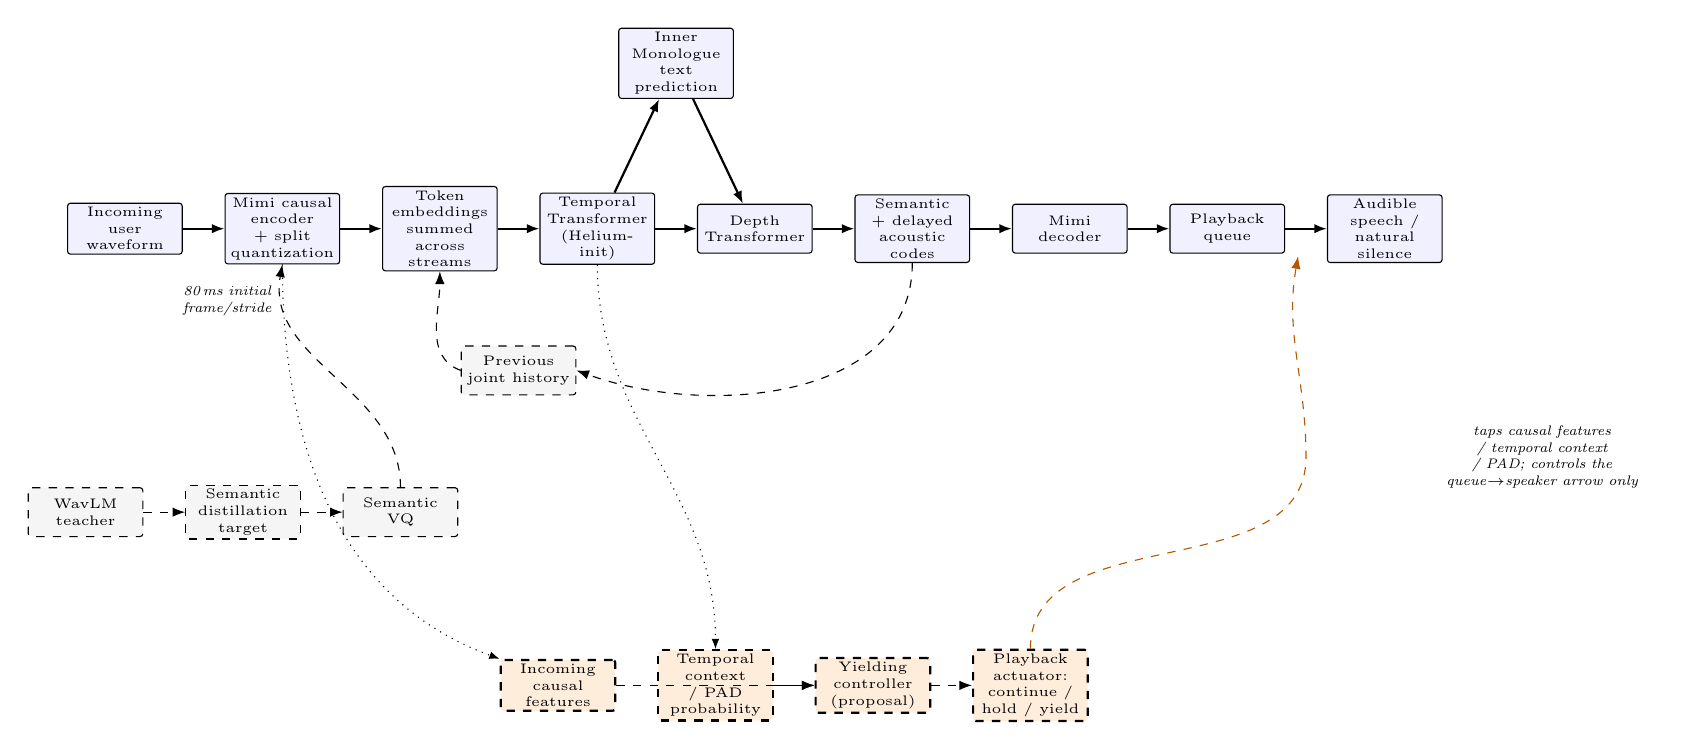
\begin{tikzpicture}
  % Panel A main chain (absolute grid: dx=2.0cm, main row y=0)
  \node[box] (a1) at (0,0) {Incoming user waveform};
  \node[box] (a2) at (2,0) {Mimi causal encoder + split quantization};
  \node[box] (a3) at (4,0) {Token embeddings summed across streams};
  \node[box] (a4) at (6,0) {Temporal Transformer (Helium-init)};
  \node[box] (a6) at (8,0) {Depth Transformer};
  \node[box] (a7) at (10,0) {Semantic + delayed acoustic codes};
  \node[box] (a8) at (12,0) {Mimi decoder};
  \node[box] (a9) at (14,0) {Playback queue};
  \node[box] (a10) at (16,0) {Audible speech / natural silence};
  \node[box] (a5) at (7,2.1) {Inner Monologue text prediction};
  \node[note, text width=2.0cm, anchor=north] at ([xshift=-0.7cm,yshift=-0.15cm]a2.south) {80\,ms initial frame/stride};

  \draw[arr] (a1) -- (a2);
  \draw[arr] (a2) -- (a3);
  \draw[arr] (a3) -- (a4);
  \draw[arr] (a4) -- (a5);
  \draw[arr] (a4) -- (a6);
  \draw[arr] (a5) -- (a6);
  \draw[arr] (a6) -- (a7);
  \draw[arr] (a7) -- (a8);
  \draw[arr] (a8) -- (a9);
  \draw[arr] (a9) -- (a10);

  % Feedback: previous joint history
  \node[dbox] (ah) at (5,-1.8) {Previous joint history};
  \draw[darr] (a7.south) to[out=-90,in=-20] (ah.east);
  \draw[darr] (ah.west) to[out=160,in=-90] (a3.south);

  % Training-only dashed branch
  \node[dbox] (wavlm) at (-0.5,-3.6) {WavLM teacher};
  \node[dbox] (distill) at (1.5,-3.6) {Semantic distillation target};
  \node[dbox] (semvq) at (3.5,-3.6) {Semantic VQ};
  \draw[darr] (wavlm) -- (distill);
  \draw[darr] (distill) -- (semvq);
  \draw[darr] (semvq.north) to[out=90,in=-100] (a2.south);

  % Proposal overlay (visually distinct, dashed orange)
  \node[pbox] (p1) at (5.5,-5.8) {Incoming causal features};
  \node[pbox] (p2) at (7.5,-5.8) {Temporal context / PAD probability};
  \node[pbox] (p3) at (9.5,-5.8) {Yielding controller (proposal)};
  \node[pbox] (p4) at (11.5,-5.8) {Playback actuator: continue / hold / yield};
  \draw[darr] (p1) -- (p3);
  \draw[darr] (p2) -- (p3);
  \draw[darr] (p3) -- (p4);
  \draw[dotarr] (a2.south) to[out=-90,in=160] (p1.north west);
  \draw[dotarr] (a4.south) to[out=-90,in=90] (p2.north);
  \draw[darr, orange!70!black] (p4.north) to[out=90,in=-90] (15,-2.9) to[out=90,in=-100] (14.9,-0.35);
  \node[note, text width=2.6cm] at (18,-2.9) {taps causal features / temporal context / PAD; controls the queue$\to$speaker arrow only};
\end{tikzpicture}}
\begin{center}\footnotesize Per-stage compute duration (encoder, Transformer, decoder, queue) is not individually reported; only the end-to-end figures above are stated. Dashed gray boxes are training-only; dashed orange boxes are the proposed controller, not an evaluated component.\end{center}

\vspace{0.4em}
\begin{center}\footnotesize\textit{Input: 2-second attention blocks (not an end-to-end latency measurement). DiT: 4-block context, 2 past + current + 1 future; future-block duration not reported.}\end{center}
\resizebox{\textwidth}{!}{%
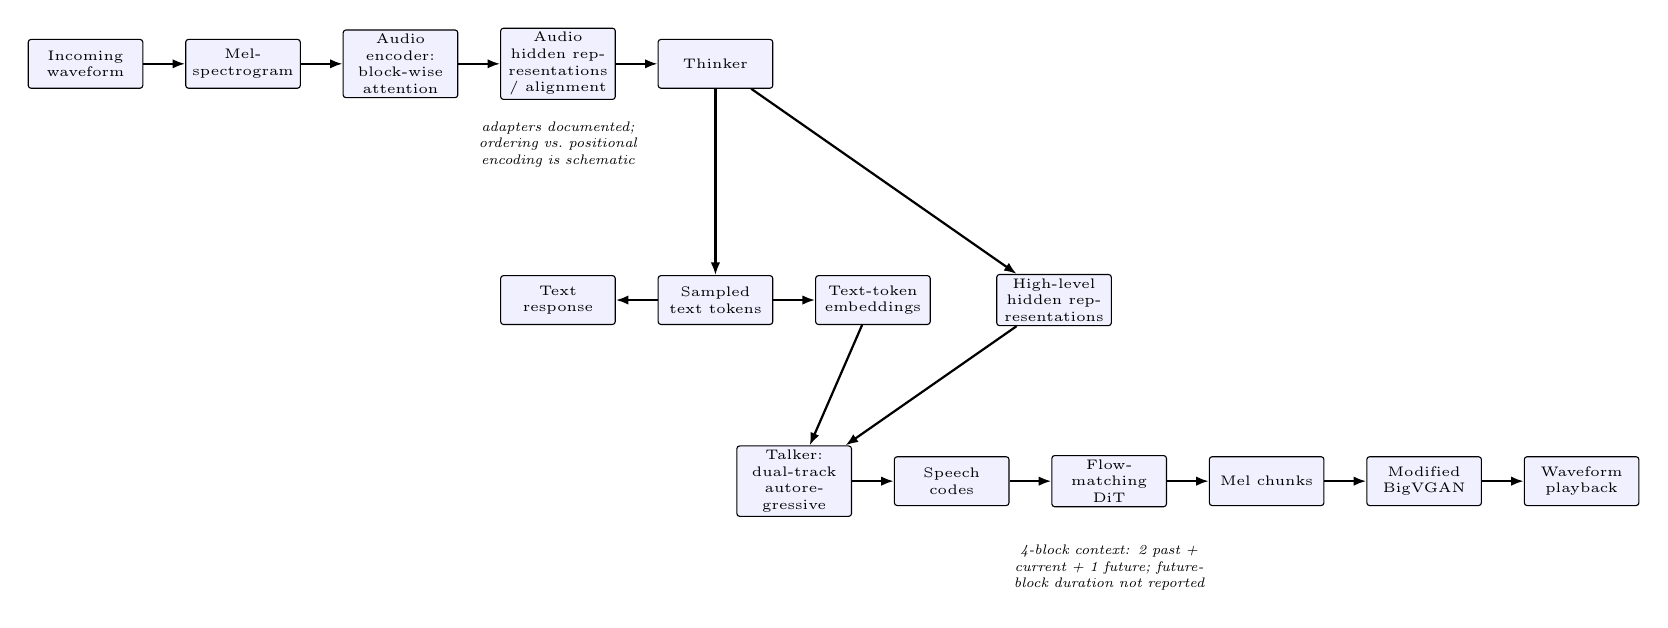
\begin{tikzpicture}
  \node[box] (b1) at (0,0) {Incoming waveform};
  \node[box] (b2) at (2,0) {Mel-spectrogram};
  \node[box] (b3) at (4,0) {Audio encoder: block-wise attention};
  \node[box] (b4) at (6,0) {Audio hidden representations / alignment};
  \node[box] (b5) at (8,0) {Thinker};
  \node[note, text width=2.6cm, anchor=north] at ([yshift=-0.15cm]b4.south) {adapters documented; ordering vs.\ positional encoding is schematic};

  \draw[arr] (b1) -- (b2);
  \draw[arr] (b2) -- (b3);
  \draw[arr] (b3) -- (b4);
  \draw[arr] (b4) -- (b5);

  \node[box] (b7) at (6,-3.0) {Text response};
  \node[box] (b6) at (8,-3.0) {Sampled text tokens};
  \node[box] (b9) at (10,-3.0) {Text-token embeddings};
  \node[box] (b8) at (12.3,-3.0) {High-level hidden representations};

  \draw[arr] (b5) -- (b6);
  \draw[arr] (b6) -- (b7);
  \draw[arr] (b6) -- (b9);
  \draw[arr] (b5) -- (b8);

  \node[box] (b10) at (9,-5.3) {Talker: dual-track autoregressive};
  \node[box] (b11) at (11,-5.3) {Speech codes};
  \node[box] (b12) at (13,-5.3) {Flow-matching DiT};
  \node[box] (b13) at (15,-5.3) {Mel chunks};
  \node[box] (b14) at (17,-5.3) {Modified BigVGAN};
  \node[box] (b15) at (19,-5.3) {Waveform playback};
  \node[note, text width=2.6cm] at (13,-6.4) {4-block context: 2 past + current + 1 future; future-block duration not reported};

  \draw[arr] (b9) -- (b10);
  \draw[arr] (b8) -- (b10);
  \draw[arr] (b10) -- (b11);
  \draw[arr] (b11) -- (b12);
  \draw[arr] (b12) -- (b13);
  \draw[arr] (b13) -- (b14);
  \draw[arr] (b14) -- (b15);
\end{tikzpicture}}
\begin{center}\footnotesize Per-stage compute duration and total onset delay are not reported in the source for either path.\end{center}
\caption{Architecture and timing dependencies. Top: Moshi (M §§3.3--3.4, pp.9--17; abstract, p.1). Bottom: Qwen2.5-Omni (Q §§2.1--2.4, pp.3--5; §3, p.6). Arrows show dependencies, not proportional execution durations. Solid = established pipeline; dashed gray = training-only path; dashed orange = the proposed yielding controller (a proposal, not a reported or evaluated component).}
\label{fig:architecture}
\end{figure}

\newpage
\section{End-of-speech is four decisions}

\begingroup
\small
\begin{longtable}{
  >{\raggedright\arraybackslash}p{3.0cm}
  >{\raggedright\arraybackslash}p{5.8cm}
  >{\raggedright\arraybackslash}p{6.1cm}
}
\toprule
\textbf{Decision} & \textbf{Operational meaning} & \textbf{Observable contrast} \\
\midrule
\endfirsthead
\toprule
\textbf{Decision} & \textbf{Operational meaning} & \textbf{Observable contrast} \\
\midrule
\endhead
\bottomrule
\endfoot
Input endpoint & User has finished the current contribution. & Hesitation pause versus completed question. \\
Conversational yield & Assistant gives the user the floor. & Backchannel versus genuine interruption. \\
Output completion & Intended response has finished playing. & Intended completion versus playback/queue state. \\
Session termination & Conversation processing stops running. & Explicit session-stop action versus ongoing listening. \\
\end{longtable}
\endgroup

Moshi establishes continuous listening and generation, including silence; PAD/EPAD concern text timing rather than a standalone utterance-stop command (M §3.4.4, pp.16-17). Qwen establishes text/message boundaries and streaming waveform generation (Q Fig.2, p.3; §§2.3-2.4, p.5; §4.1, p.6). The disclosure identifies the remaining specification boundary.

The observable test should preserve the floor through a user's hesitation, permit an answer after a completed question, continue through a non-interrupting backchannel, and yield after a genuine interruption. These are annotation targets, not assumed behaviors. A user-owned hesitation tests premature response onset; it cannot count as a false yield when the assistant has no active or pending output. Report that case separately. For hesitation episodes eligible for false-yield analysis, annotators must independently establish that the assistant should retain the floor.

\begin{figure}[htbp]
\centering
\def\lanewidth{3.9cm}
\newcommand{\eventpanel}[6]{%
  \begin{tikzpicture}[node distance=0pt]
    \tiny
    \node[lbl, text width=1.9cm, anchor=east] (l1) at (0,0) {User audio};
    \node[lbl, text width=1.9cm, anchor=east] (l2) at (0,-0.5) {Assistant audio};
    \node[lbl, text width=1.9cm, anchor=east] (l3) at (0,-1.0) {Floor ownership};
    \node[lbl, text width=1.9cm, anchor=east] (l4) at (0,-1.5) {Controller action};
    \draw[draw=gray] (0.1,0.18) rectangle (0.1+\lanewidth,-0.18) ; #1
    \draw[draw=gray] (0.1,-0.32) rectangle (0.1+\lanewidth,-0.68) ; #2
    \draw[draw=gray] (0.1,-0.82) rectangle (0.1+\lanewidth,-1.18) ; #3
    \draw[draw=gray] (0.1,-1.32) rectangle (0.1+\lanewidth,-1.68) ; #4
    \node[note, below=2mm of l4, anchor=north west, xshift=-1.85cm, text width=6.2cm] {#5};
    \node[note, below=7mm of l4, anchor=north west, xshift=-1.85cm, text width=6.2cm] {#6};
  \end{tikzpicture}%
}
\begin{minipage}{0.48\textwidth}
\centering
\footnotesize\textbf{Hesitation pause}\\[2pt]
\eventpanel{
  \fill[blue!35] (0.1,0.18) rectangle (1.3,-0.18);
  \fill[blue!35] (2.3,0.18) rectangle (3.9,-0.18);
}{
  \fill[gray!15] (0.1,-0.32) rectangle (4.0,-0.68);
}{
  \node[font=\tiny] at (2.0,-1.0) {User (throughout)};
}{
  \node[font=\tiny] at (2.0,-1.5) {Hold -- do not start};
}{Label: \textit{``Endpoint control: do not start prematurely.''}}{False-yield analysis includes only episodes with active/pending assistant output and an independently annotated assistant floor.}
\end{minipage}
\hfill
\begin{minipage}{0.48\textwidth}
\centering
\footnotesize\textbf{Backchannel}\\[2pt]
\eventpanel{
  \fill[blue!35] (1.6,0.18) rectangle (2.2,-0.18);
}{
  \fill[orange!35] (0.1,0.18) rectangle (4.0,-0.18);
}{
  \node[font=\tiny] at (2.0,-1.0) {Assistant (throughout)};
}{
  \node[font=\tiny] at (2.0,-1.5) {Continue};
}{Label: \textit{``Continue; do not yield solely because speech is detected.''}}{}
\end{minipage}

\vspace{0.6em}
\begin{minipage}{0.48\textwidth}
\centering
\footnotesize\textbf{Genuine interruption}\\[2pt]
\eventpanel{
  \fill[blue!35] (1.9,0.18) rectangle (4.0,-0.18);
}{
  \fill[orange!35] (0.1,0.18) rectangle (2.2,-0.18);
}{
  \node[font=\tiny] at (1.0,-1.0) {Assistant};
  \node[font=\tiny] at (3.0,-1.0) {User};
}{
  \node[font=\tiny] at (2.0,-1.5) {Yield};
}{Marked interval: \textit{``Interruption-to-yield latency: measured in experiment.''}}{}
\end{minipage}
\hfill
\begin{minipage}{0.48\textwidth}
\centering
\footnotesize\textbf{Completed question}\\[2pt]
\eventpanel{
  \fill[blue!35] (0.1,0.18) rectangle (2.0,-0.18);
}{
  \fill[orange!35] (2.1,0.18) rectangle (4.0,-0.18);
}{
  \node[font=\tiny] at (1.0,-1.0) {User};
  \node[font=\tiny] at (3.0,-1.0) {Assistant};
}{
  \node[font=\tiny] at (2.0,-1.5) {Answer onset};
}{Label: \textit{``Answer onset; distinct from interruption yielding.''}}{}
\end{minipage}
\caption{Conversational events and desired actions. Four lanes per panel: user audio, assistant audible audio, desired floor ownership, desired controller action. Time is symbolic (no numerical durations). These are desired behaviors for the proposed test, not measured traces.}
\label{fig:events}
\end{figure}

\section{Selected hypothesis}

\textbf{We hypothesize that a frozen speech LLM's own generation state improves continue/hold/yield decisions beyond incoming audio and observable playback history, which predicts fewer false yields on eligible backchannel and hesitation events than speech-activity rules and an audio-only learned controller, under matched interruption-to-yield latency and missed-interruption constraints.}

The hypothesis is refuted if the state-aware controller cannot improve that constrained comparison on held-out speakers and conversations, or if removing generation state preserves the benefit.

Four alternatives remain secondary: whether buffering dominates onset latency; whether codec phonetic quality predicts interaction accuracy; whether limited lookahead causes prosodic commitment errors; and whether real overlapping dialogue contributes beyond synthetic conversation training.

\newpage
\section{Proposed improvement: state-aware yielding}

\subsection{Failure mechanism and proposed change}

A speech-activity rule can interpret acknowledgment as a takeover attempt. This is a hypothesized baseline failure, not an established failure of either paper's model.

Attach a small causal controller to \textbf{frozen Moshi}. Inputs are current Mimi representations and causal speech-activity features, observable assistant playback activity, elapsed activity/silence durations, and queue occupancy. Add Moshi's Temporal Transformer context vector and self-text PAD probability as generation-state features. Temporal context and text prediction are defined in the architecture (M §3.4.1, pp.13-14; §3.4.4, pp.16-17); implementation access requires checking. Only values available at decision time enter the controller.

A learned projection and recurrent classifier produce \textbf{continue, hold, or yield}. Continue releases available audio. Hold briefly suspends release while listening continues. Yield suppresses output and clears pending playback while retaining listening; playback resumes only through a later controller decision. All variants share the same bounded actuator. Hold duration is capped on development data; inappropriate holding counts as disruption, not as a successful non-yield.

The contribution under test is the speech LLM's generation state, not turn-taking prediction itself. Base-model parameters remain frozen; controller size and runtime are measured rather than assumed negligible.

\subsection{Training and labeled data}

Train only the projection and classifier with supervised action cross-entropy. Labels identify event type, floor ownership, event onset, acceptable action intervals, and interruption-response deadlines. Annotators hear surrounding dialogue and mark ambiguity independently of controller outputs. Future context can inform annotation but cannot become an input feature.

Collect consented human-Moshi conversations and controlled reenactments, recording separate user and actually played assistant channels. Replay recordings through frozen Moshi to obtain causal feature traces. Fisher's separate channels provide a potential auxiliary source for human conversational cues (M §4.2, p.18); new action annotations and human-system validation remain necessary. Split by speaker, conversation, and scenario. Retain disagreement scores for sensitivity analysis rather than silently excluding ambiguous cases.

Select class weights, thresholds, and hold limits on development data, leaving the test set untouched. Include logged policy rollouts as well as reenactments to expose training to action histories. A pilot should establish label reliability and event coverage before fixing the evaluation population.

\subsection{Predicted effect and baselines}

The prediction is fewer inappropriate floor relinquishments without slower or less reliable interruption handling. The \textbf{speech-activity-triggered baseline} suppresses output after incoming activity satisfies an activity threshold and persistence condition. Include both a \textbf{prespecified fixed-threshold version} and a \textbf{development-tuned version}. Give tuned rules and learned controllers the same validation protocol and playback actuator. Report unmodified Moshi as context.

Winning only against the fixed rule does not establish a generation-state benefit. Winning through additional waiting does not satisfy the hypothesis. The audio-only learned condition is necessary to distinguish useful internal state from the general benefit of supervised event classification.

\newpage
\section{Experimental design and causal controls}

\subsection{Primary experiment and metric}

Use matched \textbf{backchannel, hesitation-pause, and genuine-interruption} scenarios, balancing speakers and recording conditions across systems. Infer floor intent from context, not event duration alone. Completed questions provide an endpoint sanity check outside the primary false-yield comparison.

The primary metric is the \textbf{unweighted mean of false-yield rates for eligible backchannels and hesitation episodes}, also reported separately. A false yield is suppression when floor retention is annotated. A hold exceeding the annotated tolerance counts as equivalent disruption. Publish eligibility denominators, premature starts during user-owned hesitation, and unnecessary hold time.

Compare operating points under common \textbf{interruption-to-yield latency} and \textbf{missed-interruption} limits established from development-set baseline behavior before testing. Latency runs from annotated interruption onset to actual playback cessation. Failure to yield within the annotated deadline is a miss. Report latency distributions alongside misses, never successful responses alone. If no operating point meets both constraints, the proposed benefit is unsupported. Estimate paired uncertainty by conversation, preserving within-dialogue dependence.

\begin{figure}[htbp]
\centering
\footnotesize
\begin{tabular}{c c c}
\tikz\node[draw, circle, fill=blue!15, inner sep=3pt, font=\tiny]{BC}; Backchannel &
\tikz\node[draw, circle, fill=orange!20, inner sep=3pt, font=\tiny]{HES}; Hesitation &
\tikz\node[draw, circle, fill=red!15, inner sep=3pt, font=\tiny]{INT}; Interruption \\
\end{tabular}

\vspace{0.4em}
\begin{tabular}{@{}l c c c l@{}}
\toprule
\textbf{Condition} & \textbf{Audio cues} & \textbf{Playback history} & \textbf{Moshi state} & \textbf{Threshold selection} \\
\midrule
Unmodified Moshi & Native & Native & Native & No added controller \\
Fixed speech-activity rule & Yes & Same actuator & No & Prespecified \\
Tuned speech-activity rule & Yes & Same actuator & No & Development set \\
Audio-only learned controller & Yes & Yes & No & Development set \\
State-aware learned controller & Yes & Yes & Yes & Development set \\
\bottomrule
\end{tabular}

\vspace{0.5em}
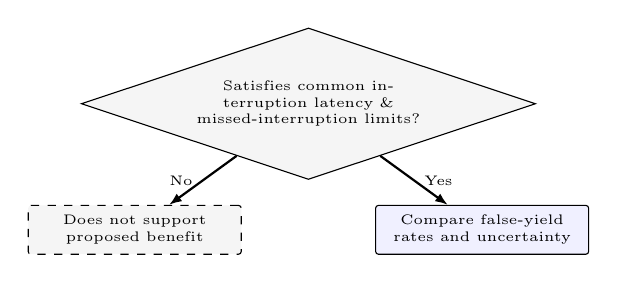
\begin{tikzpicture}[node distance=5mm]
  \node[draw, diamond, aspect=3, align=center, font=\tiny, text width=3.1cm, fill=gray!8] (gate) {Satisfies common interruption latency \& missed-interruption limits?};
  \node[dbox, below left=8mm and -6mm of gate, text width=2.6cm] (no) {Does not support proposed benefit};
  \node[box, below right=8mm and -6mm of gate, text width=2.6cm] (yes) {Compare false-yield rates and uncertainty};
  \draw[arr] (gate) -- node[left, font=\tiny] {No} (no);
  \draw[arr] (gate) -- node[right, font=\tiny] {Yes} (yes);
\end{tikzpicture}

\vspace{0.4em}
\begin{minipage}{0.47\textwidth}
\fbox{\parbox{0.92\linewidth}{\footnotesize\textbf{Held fixed:} checkpoint, generation settings, hardware, recordings, actuator, annotation protocol.}}
\end{minipage}
\hfill
\begin{minipage}{0.47\textwidth}
\fbox{\parbox{0.92\linewidth}{\footnotesize\textbf{Separate checks:} noise/echo robustness; Hindi/Telugu transfer; resumption coherence.}}
\end{minipage}
\caption{Experimental design matrix. No empirical curve is implied; all rows are proposed conditions, not measured results.}
\label{fig:matrix}
\end{figure}

\subsection{Diagnostic ablation}

Remove generation-state features while retaining acoustic features, playback history, queue state, classifier capacity, and training procedure. This tests whether a learned audio policy or knowledge that the assistant is speaking explains the gain. Both learned variants receive observable timing and playback cues; internal state must contribute beyond them. Keep the classifier architecture and training budget matched, and report any parameter-count difference introduced by the input projection.

\subsection{Robustness and Indic transfer question}

Repeat held-out events with controlled noise and echo perturbations, identical across variants. Report activity-detection and controller errors separately. A \textbf{Hindi/Telugu subset} asks whether learned cues transfer, using fluent annotators and language-specific agreement reporting. Separate adaptation from zero-shot transfer; assume no known Indic failure of either base model. Report basic instruction comprehension so lexical misunderstanding is not automatically attributed to yielding.

\subsection{What is controlled}

Fix the Moshi checkpoint, generation settings, hardware, user recordings, playback mechanism, and annotation protocol. Immediate replay comparisons start from a common assistant prefix. Counterbalance live trials where different assistant actions change user responses. The design does not control Moshi's original training history or establish causality between Moshi and Qwen architectures.

\newpage
\section{Failure modes and alternative explanations}

\textbf{Timing shortcuts.} Generation state may reveal only elapsed time or current speaking status. Supplying playback history, queue state, and durations to both learned variants tests that explanation. A benefit surviving state removal would reject the proposed contribution even if the controller still beats the rule.

\textbf{Threshold selection and extra waiting.} The development-tuned rule tests whether calibration explains an apparent gain. Common interruption constraints and explicit hold accounting test whether conservatism merely hides errors. Report the full operating-point comparison rather than selecting favorable test thresholds.

\textbf{Speaker and script shortcuts.} Speaker-disjoint splits test identity dependence. Natural held-out conversations test whether reenactment-specific lexical or prosodic cues explain performance. Language-specific disagreement and comprehension checks are needed before interpreting the Hindi/Telugu subset.

\textbf{Internal versus audible history.} Moshi can internally generate speech that suppression prevents the user from hearing. Freezing the model does not solve this mismatch. Track unheard output, resumption coherence, truncation, and controller overhead in follow-up turns. This proposal controls audible yielding; it does not repair the generator's internal dialogue state. Failure on these checks would limit or invalidate deployment despite a favorable primary metric.

\textbf{Metric sufficiency.} Fewer false yields are useful only when genuine interruptions remain responsive and subsequent conversation remains coherent. Audio quality, excessive pauses, and task completion should accompany the primary constrained metric as diagnostic outcomes, without replacing it after results are seen.

\section{Related work and contribution boundary}

\textbf{dGSLM} provides a duplex-dialogue comparison in Moshi's evaluation (M §5.6, p.31); \textbf{Mini-Omni} motivates Qwen's dual-track decoder (Q §2.1, p.3). \textbf{TurnGPT [external]} predicts conversational turn-taking [3], and \textbf{Voice Activity Projection [external]} models future conversational voice activity [4]. Turn prediction therefore predates this proposal. The narrower question is whether Moshi's own generation state adds control information beyond matched audio and playback cues. Priority for that combination requires a wider literature check; no first-use claim is made.

\section{Position}

Moshi is the justified experimental base because simultaneous listening and speaking are explicit in its formulation. Qwen demonstrates why streaming input and output alone do not establish event-level conversational decisions. The controller tests whether generation context reduces false yields without delaying genuine interruptions. Success depends on the constrained comparison, the state-removal ablation, and coherent resumption, not a lower first-audio number.

\section*{References}
\begin{enumerate}[label={[\arabic*]}, leftmargin=1.6em, itemsep=0.3em]
\item Defossez et al. \textbf{Moshi: a speech-text foundation model for real-time dialogue.} Attached arXiv:2410.00037v2, 2 October 2024.
\item Qwen Team. \textbf{Qwen2.5-Omni Technical Report.} Attached arXiv:2503.20215v1; title-page date 27 March 2025.
\item Ekstedt and Skantze. \textbf{TurnGPT: a Transformer-based Language Model for Predicting Turn-taking in Spoken Dialog.} Findings of EMNLP, 2020. \url{https://aclanthology.org/2020.findings-emnlp.268/}
\item Ekstedt and Skantze. \textbf{Voice Activity Projection: Self-supervised Learning of Turn-taking Events.} 2022. \url{https://arxiv.org/abs/2205.09812}
\end{enumerate}

\newpage
\section*{Appendix A. Detailed Moshi evidence}

\subsection*{Encoder and representation learning}

Mimi uses a SeaNet-based causal autoencoder. Four convolutional blocks with strides \textbf{(4, 5, 6, 8)} and a final convolution with stride \textbf{2} map \textbf{24\,kHz} mono audio to \textbf{512-dimensional} representations at \textbf{12.5 frames/s}. Transformer modules before and after quantization each have \textbf{8 layers and 8 heads}, with causal masking (M §3.3.1, p.10).

Mimi uses \textbf{8 codebooks}, each with \textbf{2,048 entries}, giving the reported \textbf{1.1\,kbps} at \textbf{12.5\,Hz} (M §3.3.1, p.11). Split quantization combines one semantic VQ with a \textbf{7-level} acoustic RVQ, summing their outputs for reconstruction. WavLM teacher features are \textbf{1,024-dimensional at 50\,Hz}, pooled to \textbf{12.5\,Hz}. Cosine-distance distillation uses non-causal teacher information during training while Mimi remains causal at inference (M §3.3.2, p.12).

The paper evaluates an adversarial-only codec variant retaining feature and discriminator losses alongside semantic distillation. This is a description of the evaluated variant rather than an unsupported final-configuration designation (M §3.3.1, p.11; §5.2, Table 4, p.24).

\subsection*{Alignment, generation, and streaming}

The Temporal Transformer receives summed learned embeddings across parallel sequences. The Depth Transformer conditions on temporal context and preceding within-timestep tokens (M §3.4.1, pp.13-14). Inner Monologue aligns self-text using Whisper timestamps and PAD/EPAD. User input is not mediated by a user transcript in this formulation (M §3.4.4, p.16).

The joint sequence includes both participants' audio and Moshi's text: $K = 2Q + 1$, with $Q = 8$. Actual user audio replaces predicted user-stream tokens during interaction (M §3.4.4, p.17). Mimi's initial frame and stride are \textbf{80\,ms} (M §3.3.1, p.11). The reported model latency is \textbf{160\,ms theoretical and 200\,ms practical} (M abstract, p.1). Acoustic delay is \textbf{2} during pretraining and \textbf{1} during fine-tuning (M §5.3, p.27).

Separate ASR/TTS configurations use \textbf{2 seconds} of text/audio delay; these are distinct from the conversational configuration (M §5.7, pp.31-32; Appendix C, p.56). EPAD ends padding, not an utterance; Appendix C's text \texttt{<bos>}/\texttt{<eos>} separates speakers in the multi-stream TTS setup (M §3.4.4, p.16; Appendix C, p.56).

\subsection*{Training objectives and data}

Stages are Helium pretraining, single-stream audio pretraining, simulated multi-stream post-training, Fisher fine-tuning, and synthetic instruction fine-tuning. Joint-token cross-entropy gives semantic tokens weight \textbf{100} and acoustic tokens weight \textbf{1} (M §4.4, pp.20-21, Eq.7).

Helium uses \textbf{2.1 trillion text tokens} (M §1, p.3), drawn from CommonCrawl, Wikipedia-family sources, StackExchange, and peS2o (M §4.1, p.17). Audio pretraining uses \textbf{7 million hours}, predominantly English, transcribed with Whisper-large-v3. Fisher supplies \textbf{2,000 hours} with separate conversation channels (M §4.2, p.18).

Synthetic instruction data contains \textbf{more than 20,000 hours}. A separate \textbf{170-hour} conversation collection supports TTS training and transcript preparation; Moshi is not directly trained on that audio collection (M §§4.2-4.3, p.18; §4.4, p.21). These figures do not establish a unique-data total.

\newpage
\section*{Appendix B. Qwen evidence and proposal checks}

\subsection*{Input representation and alignment}

Audio is resampled to \textbf{16\,kHz}, using a \textbf{128-channel} mel-spectrogram, \textbf{25\,ms} window, and \textbf{10\,ms} hop. Representations correspond approximately to \textbf{40\,ms} each (Q §2.2, p.4). The Qwen2-Audio encoder is initialized from Whisper-large-v3; adapters are trained before encoders against the initially frozen LLM (Q §2.2, p.4; §3, p.6).

Thinker is a Transformer decoder. Talker receives high-level representations and sampled text-token embeddings, combining semantic context with phonetic specificity (Q §2.1, p.3; §2.3, p.5). Exact adapter ordering relative to positional encoding remains schematic in Figure 1.

\subsection*{Generation and streaming}

Talker autoregressively generates text and audio without requiring word-level/timestamp-level text-speech alignment (Q §2.3, p.5). Input attention uses \textbf{2-second blocks}; audio-video time interleaving separately uses \textbf{2-second groups} (Q §2.2, p.4; §2.4, p.5).

Speech codes pass through flow-matching DiT, mel-spectrogram generation, and modified BigVGAN. DiT uses \textbf{4 blocks}, including \textbf{2 lookback blocks and 1 lookahead block} (Q §2.4, p.5). Distinguish this waveform path from Talker's autoregressive code generation.

\subsection*{Training requirements}

Pretraining freezes the LLM initially, unfreezes all parameters next, and extends context last. Second-phase additions are \textbf{800 billion image/video-related tokens}, \textbf{300 billion audio-related tokens}, and \textbf{100 billion video-with-audio-related tokens}. Context increases from \textbf{8,192 to 32,768 tokens} (Q §3, p.6).

Thinker uses text, visual, audio, and mixed-modality instruction data. Talker uses continuation next-token prediction, DPO, and multi-speaker instruction/speaker tuning. Preference ranking uses WER and punctuation-pause error (Q §§4.2-4.3, pp.6-7).

\subsection*{Annotation and causal interpretation}

Annotate event class and desired floor action separately. Establish eligibility before observing controller outcomes. Record onset, floor ownership, active/queued output, action tolerance, and interruption deadline. Keep ambiguity scores. The primary false-yield denominator excludes user-owned pauses without assistant output; those belong to premature-start analysis.

Replay tests immediate actions from a common prefix. Interactive follow-up tests whether different policies change human behavior and resumption coherence. These experiments support different conclusions and should not be merged into a single causal claim.

\subsection*{VERIFY before a novelty or implementation claim}

\textbf{[external]} Check TurnGPT's turn-prediction role against [3], and Voice Activity Projection's future-activity task against [4]. Their existence does not establish novelty of the proposed state-aware wrapper. Search for previous generation-state-based turn controllers before making a priority claim.

Check causal feature extraction, PAD-probability access, controller overhead, audible discontinuities, and mismatch between internal and played history. Confirm Fisher access and permitted use before selecting it as an annotation source. Controller architecture, supervision, metrics, thresholds, Hindi/Telugu transfer, and all expected effects are proposals, not findings from the papers.

\end{document}
